\RequirePackage{rotating}
%%%%%%%% Document Styles and Packages %%%%%%

\documentclass{amsart}  

\usepackage[foot]{amsaddr}
\usepackage[page]{appendix}

\usepackage[usenames, dvipsnames]{color}
\usepackage{amsfonts}
\usepackage{amsthm}
\usepackage{amsmath}
\usepackage{amsfonts}
\usepackage{latexsym}
\usepackage{amssymb}
\usepackage{amscd}
\usepackage[latin1]{inputenc}
\usepackage{verbatim}
\usepackage{enumerate}
\usepackage{enumitem}
\usepackage{graphicx}
\usepackage{xcolor}
%\usepackage{tkz-berge}
\usepackage{tikz}
\usepackage{tikzpagenodes}
\usepackage{caption}
\usepackage{adjustbox}
%=============================
\usepackage{algorithm2e}
\usepackage{algorithmic}
\usepackage{epstopdf}
\usepackage{fancybox}
\usepackage{booktabs} 
\usepackage{expl3}
\usepackage{l3keys2e}
\usepackage{xparse}
\usepackage{blkarray}
\usepackage{pst-node}
\usepackage{subcaption}
\usepackage{animate}
%\usepackage{tkz-graph}
\usepackage{float}
%\usepackage[table]{xcolor}
%\usepackage{kbordermatrix}
%\usepackage{nicematrix}
\usepackage{booktabs}
\usepackage{makecell}
\usepackage{systeme}
\usepackage{placeins}
\usepackage{young, pst-node}
\usepackage{blindtext}
%=============================
\usetikzlibrary{matrix}
\usetikzlibrary {positioning}
\usetikzlibrary{arrows,shapes}
\usetikzlibrary{trees}
\usetikzlibrary{backgrounds}
\usetikzlibrary{shapes.geometric}
\usetikzlibrary{calc,shapes.callouts,shapes.arrows}
\usetikzlibrary{graphs}
\usetikzlibrary{positioning, arrows}
\usetikzlibrary{fit}

%============================

\definecolor{mybluegreen}{rgb}{0.1, 0.55, 0.35}
\usepackage{caption}
\usepackage{array,booktabs}
\usepackage{rotating}
%%%%%%%%%%%%%%%%%%%%%%%%%%%%%%%%%%%

\usepackage[spaces,hyphens]{url}
\usepackage[colorlinks,allcolors=blue]{hyperref}
\setlength\defaultaddspace{0.5ex}
\usepackage[math]{cellspace}
\setlength\cellspacetoplimit{3pt}
\setlength\cellspacebottomlimit{3pt}

%%%%%%%%%%%  Environments  %%%%%%%%%%%%%%%% 

\newtheorem{theorem}{Theorem}[section]
\newtheorem{lemma}[theorem]{Lemma}
\newtheorem{proposition}[theorem]{Proposition}
\newtheorem{cor}[theorem]{Corollary}
\newtheorem{example}[theorem]{Example}
\newtheorem{conjecture}[theorem]{Conjecture} 
\newtheorem{rem}[theorem]{Remark}
\newtheorem{definition}[theorem]{Definition}
\newtheorem{conj}{Conjecture}[section]
% \newtheorem{procedure}{Procedure}[section]
\newtheorem{question}{Question}[section]
\newtheorem{quest}{Question for US}[section]
\theoremstyle{definition}
\DeclareMathOperator{\mr+}{mr_{+}}
\DeclareMathOperator{\M+}{M_{+}}
%\DeclareMathOperator{\mr}{mr}
%\DeclareMathOperator{\M}{M}
\DeclareMathOperator{\nul}{null}
\DeclareMathOperator{\tr}{tr}
\DeclareMathOperator{\one}{\bf 1}
\DeclareMathOperator{\rk}{rank}
%\newtheorem{definition}{Definition}[section]
%\newtheorem{conjecture}{Conjecture}[section]

\newcommand{\Sym}{\mathrm{Sym}} 
\newcommand{\ind}{\mathrm{ind}}
\DeclareMathOperator{\spanof}{span}

\newcommand{\Diff}[1]{D_{#1}}
\newcommand{\diff}[1]{d_{#1}}
\newcommand\fld{{\mathbb F}}
\newcommand\flde{{\mathbb E}}
\newcommand\cS{{\mathcal S}}
\newcommand\cC{{\mathbb{C}}}

\newcommand{\Mod}[1]{\ (\mathrm{mod}\ #1)}
\newcommand\bigzero{\makebox(0,0){\text{\huge0}}}

\newlength{\casewd}
\setlength{\casewd}{\widthof{\bfseries Case 0.}}%
\newlist{caseof}{enumerate}{1}
\setlist[caseof,1]{label = Case \arabic*: , wide=0pt, leftmargin=\dimexpr\casewd + \labelsep, font=\bfseries, topsep=2pt, itemsep=0pt}%

\newlist{subcaseof}{enumerate}{1}
\setlist[subcaseof,1]{label = Case \arabic*: , wide=0pt, leftmargin=\dimexpr\casewd + \labelsep, font=\bfseries, topsep=2pt, itemsep=0pt}%

%\newcommand\HMD{Weakly Hadamardable}
\definecolor{mybluegreen}{rgb}{0.1, 0.55, 0.35}
%______________________________________________________________
%~~~~~~~~~~~~~~~~~~~~~~~~~~~~~~~~~~~~~~~~~~~~~~~~~~~~~~~~~~~~~~
\title[]{Exploring perfect binary trees with relation to the HK-property}

\author[Atishaya Maharjan]{Atishaya Maharjan} \email[Atishaya Maharjan]{maharjaa@myumanitoba.ca}
\author[M.~N.~Shirazi]{Mahsa N. Shirazi} \email[M.~N.~Shirazi]{mahsa.nasrollahi@gmail.com}
\address{Department of Mathematics, University of Manitoba, Winnipeg,  R3T 2N2,
Canada}


\date{\today}

\keywords{EKR, HK-property, Perfect binary trees, Independence number}
\subjclass[2010]{%05E30, 05C50, 05C25
}

\begin{document}

%______________________________________________________________
%~~~~~~~~~~~~~~~~~~~~~~~~~~~~~~~~~~~~~~~~~~~~~~~~~~~~~~~~~~~~~~
\begin{abstract}
  A perfect binary tree is a full binary tree in which all leaves have the same depth. A set of cocliques of size $k$ ($k$-coclique) in a graph, containing a fixed vertex $v$ is called a star, and is denoted by $\mathcal{I}^n_G(v)$. We study the size of stars for different vertices in a perfect binary tree. This structure is useful in studying the Erd\H{o}s-Ko-Rado theorem. Hurbert and Kumar conjectured that in trees, the largest stars are on the leaves. The conjecture was shown to be false independently by Baber, Borg, and Feghali, Johnson and Thomas. However, in some classes of trees such as caterpillars, the conjecture holds true. In this paper, we study the perfect binary trees through the lens of star centers and seek to answer if the HK-property holds for perfect binary trees. We also aim to expand the definition of the flip function mentioned by Estrugo and Passtine in the context of perfect binary trees. We then use an algorithm by Niskanen and R. J. to generate all cocliques of a perfect binary tree of depth $d$ and compare the number of $k$-cocliques containing a vertex $v$ and a leaf $l$ to see if the HK-property holds for perfect binary trees.
\end{abstract}

%______________________________________________________________
%~~~~~~~~~~~~~~~~~~~~~~~~~~~~~~~~~~~~~~~~~~~~~~~~~~~~~~~~~~~~~~
\maketitle

%______________________________________________________________
%~~~~~~~~~~~~~~~~~~~~~~~~~~~~~~~~~~~~~~~~~~~~~~~~~~~~~~~~~~~~~~
\section{Introduction and Preliminaries}
For a given graph $G = (V,E)$, $V(G)$ and $E(G)$ denotes the vertex sets and edge sets of the graph $G$. For an arbitrary vertex, $v \in V(G)$, all vertices adjacent to $v$ are called the neighbours of $v$ and the set of neighbours of $v$ is denoted by $N_G(v)$. The degree of a vertex $v \in V(G)$ is the cardinality of the set of neighbours of $v$, and is denoted by $deg_G(v)$.

For $n \in \mathbb{Z^+}$ such that  $0 \leq n \leq |V(G)|$, a path of length $n$ in $G$ is a sequence of distinct vertices $v_1, v_2, \ldots, v_n$ such that $v_i$ is adjacent to $v_{i+1}$ for $1 \leq i \leq n-1$ and it is called a $uv$-path. A cycle is an extension of a path such that the last vertex is connected to the first vertex, i.e for a path of length $n$, $v_nv_i \in E(G)$. As such, the length of the cycle is $n + 1$.

A connected graph is a graph if for all $u,v \in V(G)$, there exists a $uv$-path. A coclique is a set of vertices such that no two vertices in the set are adjacent to each other. We denote a family of indpendent sets of a graph $G$ by $I_G$. A family of coclique of size $n$ in a graph $G$ is denoted by $\mathcal{I}^n_G$. For $v \in V(G)$, the family of indpendent sets, $\mathcal{I}^n_G(v) := \{A \in \mathcal{I}^n_G : v \in A\}$ is called a star of $\mathcal{I}^n_G$ and $v$ is called its center.

A tree is a connected graph with no cycles, it is denoted by $T$. For a vertex $v \in V(T)$, if $deg_T(v) = 1$, it is called a leaf. A vertex that is not a leaf is called an interior vertex. The vertex at the top which branches $2$ children is called the root vertex and is denoted by $Root$. The depth of a vertex is defined as the cardinality of the set of vertices of the path from the root vertex to it. The parent of a vertex $v$ is the vertex connected to $v$ on the path to $Root$. A child of a vertex $v$ is a vertex of which $v$ is the parent. We study a more particular class of trees called binary trees, denoted by $T_B$, where each interior vertex $v$ has exactly $2$ children and all leaves have the same depth. Further, a perfect binary tree is a binary tree in which every vertex $v \in V(T)$ has either $0$ or $2$ children. A perfect binary tree is denoted by $T_{PB}$, however in this paper we will simply drop the subscript and denote it as $T$ for clarity. A level $n$ of a perfect binary tree is a set of vertices such that all vertices in the set have a depth of $n$.

The star centers of a graph are interesting because they relate to the EKR theorem. 


The Erd\H{o}s-Ko-Rado (EKR) theorem limits the number of sets in a family of sets that can be pairwise intersecting. The theorem states that for a family of $k$-sets of a ground set of size $n$, the maximum number of sets that can be pairwise intersecting is $\binom{n-1}{k-1}$. This theorem has wide applications in combinatorics, graph theory, probability, and other areas of statistics and mathematics.

Studying the EKR theorem, ~\cite{MR2763040} Hulbert and Kamat tried to narrow it down to a more reduced class of graphs called the k-EKR graphs. A graph $G$ is said to be $k$-EKR if for any family of cocliques $\mathcal{F} \subset \mathcal{I}^k_G$ satisfying $A \cap B \neq \emptyset$ for every $A, B \in \mathcal{F}$, there is a vertex $x \in V(G)$ such that $|\mathcal{F}| \leq \mathcal{I}^k_G(v)$. They then conjectured the following:

\begin{conjecture}[k-EKR Conjecture]
	Let $G$ be a graph, and let $\mu(G)$ be the size of its smallest maximal coclique. Then $G$ is $k$-EKR for every $1 \leq k \leq \frac{\mu(G)}{2}$.
\end{conjecture}

However, this conjecture is hard to understand and prove, so they narrowed the class of graphs to be trees and gave the following conjecture:

\begin{conjecture}[HK-Property]
	For any $k \geq 1$ and any tree $T$, there exists a leaf $l$ of $T$ such that $|\mathcal{I}^k_T(v)| \leq |\mathcal{I}^k_T(l)|$ for each $v \in V(T)$.
\end{conjecture}

The HK-property holds true for $k \leq 4$, but was proven false independetly in ~\cite{MR3271819, MR3612439, MR2523796}. The counterexample that that they arrived at is a type of graph that is defined as a class of trees called $lobster$ ~\cite{MR4245360}.
A tree $C$ is called a $caterpillar$ if $G$ removing the leaves and incident edges produces a path graph $P$, called the spine. A tree $L$ is called a $lobster$ if removing the leaves and incident edges produces a caterpillar $C$.

This is interesting for us as $lobster$ graphs resemble a binary tree.

\begin{figure}
	\centering
	\begin{tikzpicture}[scale=0.7,level distance=2cm,
			level 1/.style={sibling distance=8cm},
			level 2/.style={sibling distance=4cm},
			level 3/.style={sibling distance=2cm},
			every node/.style={circle, draw, fill=white, minimum size=1.75em},]
		\node (v11) {$v_0$}
		child {node (v21) {$v_1$}
				child {node  {}
						child {node {}}
					}
				child {node (v32) {}
						child {node {}}
					}
			}
		child {node (v22) {$v_2$}
				child {node (v33) {}
						child {node {}}
					}
				child {node (v34) {}
						child {node {}}
					}
			};
	\end{tikzpicture}
	\caption{The largest k-star for $k \geq 5$ is centered at $v_0$ (A lobster)}
\end{figure}

They figured out that the lobsters, while not completely obeying the HK-property, almost obey the HK-property by either having the largest stars centered around the leaves or at the root of the tree.

From the EKR theorems, Holroyd and Talbot, \cite{MR2763040}, introduced the HK-property:

\begin{conj}[HK-property]
  For any k $\geq$ 1 and any tree T, there exists a leaf l of T such that $\left|\mathcal{I}^n_T(v)\right| \leq \left|\mathcal{I}^n_T(l)\right|$ for each $v \in V(T)$.
\end{conj}

This was in order to hopefully aid in the study of the EKR property which Holroyd and Talbot \cite{MR2136060} conjectured as follows:

\begin{theorem}[k-EKR]
  Let G be a graph, and let $\mu(G)$ be the size of its smallest maximal coclique. Then G is k-EKR for every 1 $\leq$ k $\leq$ $\frac{\mu(G)}{2}$
\end{theorem}

The HK-property holds true for $k \leq 4$, but was proven false independetly by ~\cite{MR3271819, MR3612439, MR2523796}. The counterexample that that they arrived at is a type of graph that is defined as a class of trees called "lobsters" ~\cite{MR4245360}. This is interesting for this paper as the counterexample graph resembles a binary tree.

In this paper, we study perfect binary trees through the lens of star centers and seek to answer if the HK-property holds for perfect binary trees. This topic is fascinating due to the lobster being a part of the binary tree class. So this begs the question whether or not perfect binary trees or other classes of binary trees admit the HK-property. In our exploration, we also aim to expand the definition of the flip function, introduced in ~\cite{MR2763040}, to accomodate the presence of escape paths in perfect binary trees. We call this function the diagonal flip function, represented by $Diag_{f}$. In the event that the perfect binary tree does not admit the HK-property, we aim to find a counterexample.

%~~~~~~~~~~~~~~~~~~~~~~~~~~~~~~~~~~~~~~~~~~~~~~~~~~~~~~~~~~~~~~
\section{Some classes of graphs that are HK and a counterexample}

In the paper by Estrugo and Passtine~\cite{MR4245360}, they gave a couple of classes of graphs that have the HK-property. The classes of graphs that they gave were the caterpillars and the stars.

\begin{figure}[htb!]
	\begin{minipage}{0.5\textwidth}
		\centering
		\begin{tikzpicture}[every node/.style={circle, draw, fill=white, minimum size=1.75em}]
			% Draw the path (spine)
			\node (v1) at (0,0) {$v_1$};
			\node (v2) at (2,0) {$v_2$};
			\node (v3) at (4,0) {$v_3$};
			\node (v4) at (6,0) {$v_4$};
			\draw (v1) -- (v2) -- (v3) -- (v4);

			% Draw the leaves
			\node (v7) at (4,2) {$v_7$};
			\node (v8) at (6,2) {$v_8$};
			\node (v9) at (6,-2) {$v_9$};  % New vertex attached to v4
			\draw (v3) -- (v7);
			\draw (v4) -- (v8);
			\draw (v4) -- (v9);  % Edge to the new vertex
		\end{tikzpicture}
		\caption{A caterpillar}
	\end{minipage}
	\begin{minipage}{0.5\textwidth}
		\centering
		\begin{tikzpicture}[every node/.style={circle, draw, fill=white, minimum size=1.75em}]
			% Draw the path (spine)
			\node (v1) at (0,0) {$v_1$};
			\node (v2) at (2,0) {$v_2$};
			\node (v3) at (4,0) {$v_3$};
			\node (v4) at (6,0) {$v_4$};
			\draw (v1) -- (v2) -- (v3) -- (v4);

			% Draw the leaves
			\node (v7) at (1,1.33) {$v_7$};
			\node (v8) at (3,1.33) {$v_8$};
			\node (v9) at (1,-1.33) {$v_9$};
			\node (v10) at (3,-1.33) {$v_{10}$};
			\draw (v2) -- (v7);
			\draw (v2) -- (v8);
			\draw (v2) -- (v9);
			\draw (v2) -- (v10);
		\end{tikzpicture}
		\caption{A Spider}
	\end{minipage}
\end{figure}

The caterpillars are trees that have a path as the spine and the leaves are attached to the spine. The spiders are trees that only have 1 vertex with degree greater than 2.

%~~~~~~~~~~~~~~~~~~~~~~~~~~~~~~~~~~~~~~~~~~~~~~~~~~~~~~~~~~~~~~
\section{Perfect Binary Trees are HK}

\begin{definition}[Maximum Coclique]
	We denote the maximum coclique of a perfect binary tree of depth $d$ by $\mathcal{I}_d$.
\end{definition}

\begin{conjecture}[HK property for a perfect binary tree]
	For any given perfect binary tree $T$, the maximum number of cocliques lie in the leaves. The number of cocliques is denoted by $k$. $\alpha(T)$ denotes the independence number of a tree $T$.
\end{conjecture}

\begin{lemma}\label{independence_num}
	For a given perfect binary tree $T$ with depth $d$ and maximum number of cocliques possible, i.e. $k = \alpha(T)$ we have:
	\begin{align*}
		\alpha(T) = \begin{cases}
			            2^{d - 1} + 2^{d-3} + \ldots + 1 \text{ for odd $d$}  \\
			            2^{d - 1} + 2^{d-3} + \ldots + 2 \text{ for even $d$} \\
		            \end{cases}
	\end{align*}

	And for odd $d$, $Root \in \mathcal{I}_d$, otherwise $Root \not\in \mathcal{I}_d$.

	Or, in summation notation:
	\begin{align*}
		\alpha(T) = \sum_{i= 0}^{\left\lfloor\frac{d}{2}\right\rfloor} 2^{d - 2i - 1}
	\end{align*}
\end{lemma}

\begin{proof}
	$ $ \\
	We shall proceed by inducing on $d$.\\
	We will have two cases, one for $d$ being odd and another for $d$ being even.
	\begin{caseof}
		\item $d$ is odd \\

		For our base case, consider the trivial case of $d = 1$. Here, $\alpha(T) = 1$. Hence, the base case holds. \\

		Now, say that the statement holds for all $d$. We now have to show that it holds for $d+1$. That is, we need to show that it holds for a given perfect binary tree $T$ of depth $d + 1$. Note that if $d$ is odd, then $d + 1$ is even. Hence, we expect that:

		\begin{align*}
			\alpha(T) = 2^d + 2^{d - 2} + \ldots + 2 
		\end{align*}

		Consider these 2 cases:

		\begin{subcaseof}
			\item $Root \in \mathcal{I}_{d + 1}$

			Let the left and right child of the root be $v_0$ and $v_1$ respectively.

			Let $C_1, C_2, C_3, C_4$ be the four perfect binary tree components generated by $T \setminus \{Root, v_0, v_1\}$.

			If the root $\in \mathcal{I}_{d + 1}$, then $v_0 \not\in \mathcal{I}_d$ and $v_1 \not\in \mathcal{I}_d$. This means that the remaining vertices of $\mathcal{I}_d$ is in one of the 4 components.
			Since the current depth from the $Root$ is $d + 1$, then $T \setminus \{Root, v_0, v_1\}$ will have depth of $d + 1 - 2 = d - 1$. Since $d$ is odd, then $d + 1$ is even which implies that $d - 1$ is also even.

			By symmetry, it is enough to consider one of the 4 components' maximum coclique for our calculations. Since the 4 components are disjoint, then we can add their independence numbers together along with the $Root$ and obtain the following:
			\begin{align*}
				\alpha(T_{d + 1}) = 4(\alpha(T_{d - 1})) + 1
			\end{align*}

			Then, from our induction hypothesis, we get that:

			\begin{align}
				\alpha(T_{d+1}) & = 4\underbrace{(2^{d - 2} + 2^{d - 4} + \ldots + 2)}_{\frac{d-1}{2} \text{terms}} + 1                           \nonumber \\
						& = 4 \displaystyle\sum_{i = 1}^{\frac{d-1}{2}}2^{d - 2i} + 1 	
			\label{eq:odd_case}
			\end{align}


		\item Root $\not\in \mathcal{I}_{d + 1}$

			If $Root \not\in \mathcal{I}_d$, then the remaining elements of $\mathcal{I}_d$ are from $T \setminus \{Root\}$.

			Let $T' = T\setminus\{Root\}$. Then $T'$ is a forest of 2 disjoint and distinct components. Let $C_1$ and $C_2$ be the 2 components of $T'$. Since $T$ was a perfect binary tree of depth $d + 1$, then $C_1$ and $C_2$ are also perfect binary trees of depth:
			\begin{align*}
				 & = (d + 1) - 1 \\
				 & = d
			\end{align*}

			Since $d$ is odd, and $C_1$ and $C_2$ are disjoint and distrinct perfect binary trees,
			\begin{align*}
				\alpha(T') = \alpha(C_1) + \alpha(C_1)
			\end{align*}

			By symmetry we get that,
			\begin{align*}
				\alpha(T') = 2\alpha(C_1)
			\end{align*}

			Since $Root \not\in \mathcal{I}_d$,
			\begin{align*}
				\alpha(T) = \alpha(T') = 2\alpha(C_1)
			\end{align*}

			Then, by our induction hypothesis,
			\begin{align}
				\alpha(T) & = \underbrace{2(2^{d - 1} + 2^{d - 3} + \dots + 1)}_{\left\lceil\frac{d}{2}\right\rceil \text{terms}}          \nonumber \\
					  & = 2\left(\displaystyle\sum_{i = 1}^{\left\lceil\frac{d}{2}\right\rceil}2^{d - (2i - 1)}\right) \nonumber
			\end{align}

			Note that $\left\lceil\frac{d}{2}\right\rceil = \frac{d + 1}{2}$, since $d$ is odd, then,
			\begin{align}
				\alpha(T) & = 2\left(\displaystyle\sum_{i = 1}^{\left\lceil\frac{d}{2}\right\rceil}2^{d - (2i - 1)}\right) \nonumber \\
					  & = 2\left(\displaystyle\sum_{i = 1}^{\frac{d + 1}{2}}2^{d - (2i - 1)}\right)  \label{eq:even_case} 
			\end{align}


		\end{subcaseof}

		Since $\alpha(T)$ is the maximum coclique,
		\begin{align*}
			\alpha(T) = \max(\ref{eq:odd_case}, \ref{eq:even_case})
		\end{align*}

		Remember that our objective is to show that $\alpha(T) = (\ref{eq:even_case})$ as this aligns with our inductive hypothesis.

		From (\ref{eq:even_case}), we can simplify it as the following:

		\begin{align*}
			\alpha(T) & = 2\left(\displaystyle\sum_{i = 1}^{\frac{d + 1}{2}}2^{d - (2i - 1)}\right)  \\
				  & = 2\left(2^{d - 2\left(\frac{d + 1}{2}\right) + 1} + \displaystyle\sum_{i = 1}^{\frac{d - 1}{2}}2^{d - (2i - 1)}\right)\\
				  & = 2\left(2^{d - d - 1 + 1} + \displaystyle\sum_{i = 1}^{\frac{d - 1}{2}}2^{d - (2i - 1)}\right)\\
				  & = 2\left(2^0 + \displaystyle\sum_{i = 1}^{\frac{d - 1}{2}}2^{d - (2i - 1)}\right)\\
				  & = 2\left(1 + \displaystyle\sum_{i = 1}^{\frac{d - 1}{2}}2^{d - (2i - 1)}\right)\\
				  & = 2\left(1 + \displaystyle\sum_{i = 1}^{\frac{d - 1}{2}}2^{d - 2i + 1)}\right)\\
				  & = 2\left(1 + 2\displaystyle\sum_{i = 1}^{\frac{d - 1}{2}}2^{d - 2i)}\right)\\
				  & = 2 + 4\displaystyle\sum_{i = 1}^{\frac{d - 1}{2}}2^{d - 2i}\\
				  & = 4\displaystyle\sum_{i = 1}^{\frac{d - 1}{2}}2^{d - 2i} + 2 \\
				  & > 4\displaystyle\sum_{i = 1}^{\frac{d - 1}{2}}2^{d - 2i} + 1 \\
				  & = (\ref{eq:odd_case})
		\end{align*}

		Which implies that,

		\begin{align*}
			\alpha(T) = \max(\ref{eq:odd_case}, \ref{eq:even_case}) = (\ref{eq:even_case})\; \text{as required.}
		\end{align*}

	\item $d$ is even \\

		We will proceed similarly to the odd case.

		For our base case, consider the case of $d = 2$. Let $v_0$ and $v_1$ be the leaves of the perfect binary tree of depth $2$. We claim that $\mathcal{I}_2 = \{v_0, v_1\}$. This implies that $Root \not\in \mathcal{I}_2$. 

		We will prove the claim by using contradiction.	

		For contradiction, say that $Root \in \mathcal{I}_2$, then $v_0 \not\in \mathcal{I}_2$ and $v_0 \not\in \mathcal{I}_2$ since both $v_0$ and $v_1$ are neighbours of $Root$. This then implies that $\alpha(T) = 1$. However, the set of leaves $\{v_0, v_1\}$ has cardinality $2 > 1 = \alpha(T)$ which is a contradiction.

		Hence, for a perfect binary tree $T$ of depth $2$, $\alpha(T) = 2$. Thus, our base case holds.


		Now, say that the statement holds for all $d$. We now have to show that it holds for $d+1$. That is, we need to show that it holds for a given perfect binary tree $T$ of depth $d + 1$. Note that if $d$ is even, then $d + 1$ is odd. Hence, we expect that:

		\begin{align*}
			\alpha(T) = 2^d + 2^{d - 2} + \ldots + 1
		\end{align*}

		which follows from our previous case.
	\end{caseof}
\end{proof}

\begin{lemma}
Following from the previous lemma ~\ref{independence_num}, we claim that if $|\mathcal{I}_d| = \alpha(T)$, then $\mathcal{I}_d$ is unique.
\end{lemma}
\begin{proof}
	$ $ \\
	Let $\mathcal{I}_d$ be the maximum coclique, we will first construct a set of vertices that build $\mathcal{I}_d$ and then show that no other vertex can be added to the set nor removed which will satisfy uniqueness.

	We shall proceed by cases.
	\begin{caseof}
	\item $d$ is odd \\
		From ~\ref{independence_num}, we know that if $d$ is odd, then $Root \in \mathcal{I}_d$. 

		Let $v_0$ and $v_1$ be the children of $Root$, 

		If $Root \in \mathcal{I}_d$, then we know that $v_0 \not\in \mathcal{I}_d$ and $v_1 \not\in \mathcal{I}_d$.

		Let $T_1, T_2, T_3, T_4$ be the disjoint components obtained from $T\setminus\{v_0, v_1, Root\}$. Note that $T_1, T_2, T_3, \text{and } T_4$ are all perfect binary trees of depth $d - 2$.

		Since $d$ was odd, then $d - 2$ is also odd.
	\end{caseof}
\end{proof}

%~~~~~~~~~~~~~~~~~~~~~~~~~~~~~~~~~~~~~~~~~~~~~~~~~~~~~~~~~~~~~~
\begin{appendix}
\section{cocliques Algorithm and Analysis}\label{coclique-algorithm}
$ $
To validate our conjecture, we present a simple algorithm to generate all cocliques of a perfect binary tree of cardinality $k$. We then compare the number of cocliques containing a vertex $v$ and a leaf $l$ to see if the HK-property holds for perfect binary trees.

To begin with, we present the following algorithm to generate a perfect binary tree of depth $n$:

\RestyleAlgo{ruled}

\SetKwComment{Comment}{/* }{ */}

\begin{algorithm}[hbt!]
  \caption{Perfect Binary Tree Generator}\label{alg:tree-generator}
  \KwData{$n \geq 0$, where $n$ is the depth of the perfect binary tree}
  \KwResult{A perfect binary tree graph and its leaves}

  \SetKwFunction{FMain}{perfect\_binary\_tree\_generator}
  \SetKwFunction{FSub}{get\_leaves}

  \SetKwProg{Fn}{Function}{:}{}
  \Fn{\FMain{$n$}}{
    \eIf{$n = 0$}{
      \Return{Graph()}
    }{
      $g \gets Graph()$\;
      $g$.add\_vertices([$2^n$])\;
      \For{$i$ in range($2^n - 1$)}{
        $g$.add\_edge($i$, $2*i + 1$)\;
        $g$.add\_edge($i$, $2*i + 2$)\;
      }
      \Return{$g$}
    }
  }
\end{algorithm}

The algorithm will generate a perfect binary tree of this form:
\begin{figure}[hbt!]
  \centering

  \begin{tikzpicture}[scale=0.7,level distance=2cm,
      level 1/.style={sibling distance=8cm},
      level 2/.style={sibling distance=4cm},
      level 3/.style={sibling distance=2cm},
      every node/.style={circle, draw, fill=white}]
    \node (0) {$0$}
    child {node (1) {$1$}
        child {node (3) {$3$}
            child {node {$\vdots$}}
            child {node {$\vdots$}}
          }
        child {node (4) {$4$}
            child {node {$\vdots$}}
            child {node {$\vdots$}}
          }
      }
    child {node (2) {$2$}
        child {node (5) {$5$}
            child {node {$\vdots$}}
            child {node {$\vdots$}}
          }
        child {node (6) {$6$}
            child {node {$\vdots$}}
            child {node {$\vdots$}}
          }
      };
  \end{tikzpicture}
\end{figure}

It is easy to see that the leaves will start with the value of $\left\lfloor\dfrac{2^{n + 1} - 1}{2}\right\rfloor$, where $n$ is the depth of the perfect binary tree.

\newpage
So to generate all the leaves of the perfect binary tree of depth $n$, we present the following algorithm:

\begin{algorithm}[hbt!]
  \caption{Perfect Binary Tree Leaves Generator}\label{alg:leaves-generator}
  \KwData{$n \geq 0$, where $n$ is the depth of the perfect binary tree}
  \KwResult{A perfect binary tree graph's leaves}

  \SetKwFunction{FMain}{perfect\_binary\_tree\_generator}

  \SetKwProg{Fn}{Function}{:}{}
  \Fn{\FMain{$n$}}{
    $num\_vertices \gets 2^{n + 1} - 1$\;
    $leaves \gets []$\;
    $last\_row\_start \gets floor(num\_vertices / 2)$\;
    \For{$vertex$ in range($last\_row\_start$, $num\_vertices$)}{
      $leaves$.append($vertex$)\;
    }
    \Return{$leaves$}
  }
\end{algorithm}

We then use the algorithm from ~\cite{Niskanen2003CliquerUG} to generate a coclique of maximum cardinality for our perfect binary tree.

\begin{algorithm}[hbt!]
  \caption{Maximum Indpendent Set Algorithm}\label{alg:max-independent-set}
  \KwData{A perfect binary tree graph $T$}
  \KwResult{A maximum coclique of $T$}

  \SetKwFunction{FMain}{maximum\_independent\_set}

  \SetKwProg{Fn}{Function}{:}{}
  \Fn{\FMain{$T$}}{
    $cliquer \gets Cliquer(T)$\;
    \Return{$cliquer$.get\_maximum\_independent\_set()}
  }
\end{algorithm}


The next page shows the results of the algorithm for a perfect binary tree of depth 5. The X-axis denotes the vertice's labels (not the actual numbers) and the Y-axis denotes the cardinality of the stars centered around the vertices.

\begin{figure}[hbt!]
	\begin{subfigure}{.5\textwidth}
		\centering
		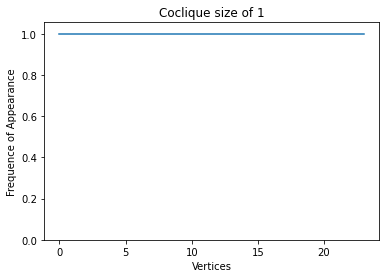
\includegraphics[width=1\linewidth]{size_1.png}
		\caption{coclique of size 1}
	\end{subfigure}
	\begin{subfigure}{.5\textwidth}
		\centering
		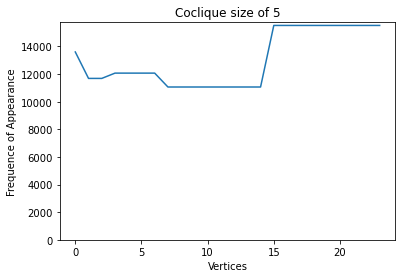
\includegraphics[width=1\linewidth]{size_5.png}
		\caption{coclique of size 5}
	\end{subfigure}
	\begin{subfigure}{.5\textwidth}
		\centering
		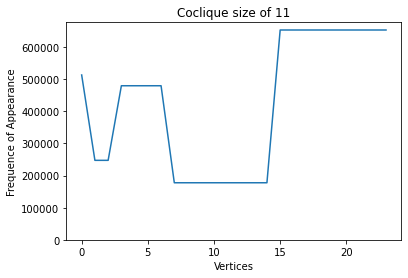
\includegraphics[width=1\linewidth]{size_11.png}
		\caption{coclique of size 11}
	\end{subfigure}
	\begin{subfigure}{.5\textwidth}
		\centering
		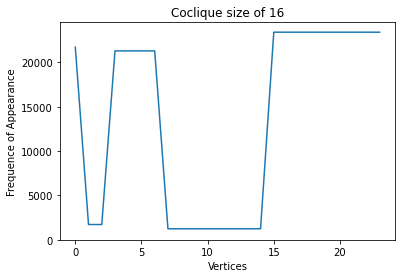
\includegraphics[width=1\linewidth]{size_16.png}
		\caption{coclique of size 16}
	\end{subfigure}
	\begin{subfigure}{.5\textwidth}
		\centering
		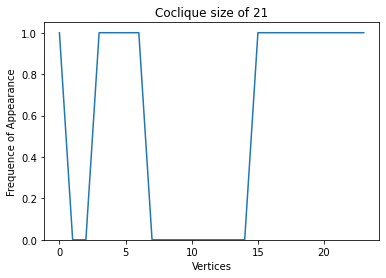
\includegraphics[width=1\linewidth]{size_21.png}
		\caption{coclique of size 21}
	\end{subfigure}
\end{figure}

The data shown in the figures above verifies that the Partial HK-Property holds for perfect binary trees of depth 5. The next step would be to verify this for perfect binary trees of depth 6 and 7.

However, the algorithm is very slow and inefficient and it scaled exponentially. Hence, running the algorithm for perfect binary trees of depth 6 and 7 would be very computationally expensive.

\end{appendix}

\newpage
%______________________________________________________________
%~~~~~~~~~~~~~~~~~~~~~~~~~~~~~~~~~~~~~~~~~~~~~~~~~~~~~~~~~~~~~~

\include{Bibliography}
\bibliographystyle{plain}
\addcontentsline{toc}{chapter}{Bibliography}
\bibliography{Bibliography}

%______________________________________________________________
%~~~~~~~~~~~~~~~~~~~~~~~~~~~~~~~~~~~~~~~~~~~~~~~~~~~~~~~~~~~~~~
\end{document}
